\section{Iteration \#2 -- Pyramid Tree and Other Hash-Based Approaches}

TODO
\begin{itemize}
	\item TODO
\end{itemize}

\subsection{Pyramid Tree}

As described in Section \ref{sec:pyramid-tree}, the Pyramid tree reduces multi-dimensional points to one dimension, which can then be used in a one-dimensional index structure. This reduction to a one-dimensional value can be seen as a hashing function, which can be used to generate search keys for the underlying hash map in the Bucket Pseudo-Pyramid Tree.

To elaborate on the reduction technique, the Pyramid tree partitions the data space into $2d$ Pyramids, where each is represented the $(d - 1)$ hyperplane corresponding to the Pyramid's base. Each pyramid is is segmented by splitting them along $(d-1)$ hyperplanes parallel to the base of the pyramid. The one-dimensional value of a point, called the \textit{pyramid value}, describes which Pyramid it is in and the height of that point in that Pyramid. The resultant spatial partition looks like Figure \ref{fig:pyramid-tree-buckets}, where each Pyramid segment has a corresponding bucket which stores the points.

\begin{figure}
		\begin{center}
			\begin{subfloat}[$2d$ Pyramids in 2D Data Space\label{fig:pyramid-tree-pyramids}]{%
				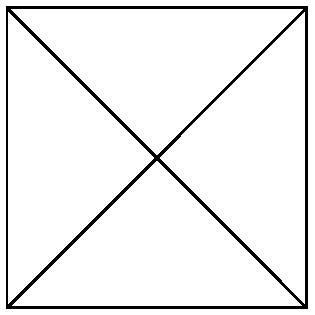
\includegraphics[scale=0.5]{figures/pyramid_tree_partition.pdf}
			}
			\end{subfloat}~
			\begin{subfloat}[Segmented $2d$ Pyramids, Each Associated with a Bucket\label{fig:pyramid-tree-buckets}] {%
				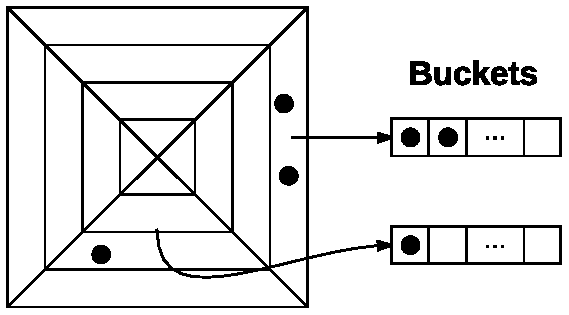
\includegraphics[scale=0.5]{figures/pyramid_tree_buckets.pdf}
			}
			\end{subfloat}
		\end{center}

		\label{fig:pyramid-tree-partition}
\end{figure}

More formally, the pyramid value $pv_v$ of a point $v$ is given by $pv_v = (i + h_v)$, where $i$ represents the pyramid $v$ is contained in and $h_v$ is height of $v$ in pyramid $i$. $i$ and $h_v$ are given in Equations \ref{eq:pyramid-value-index} and \ref{eq:pyramid-value-height} respectively, where $MOD$ refers to the modulo operator.

\begin{multline}\\
	i = \begin{cases}
		j_{max},         & \text{if }v_{j_{max}} < 0.5\\
		j_{max} + d,   & \text{if }v_{j_{max}} \geq 0.5\\
	\end{cases} \\
	j_{max} = \left( j \;|\; \forall k \; 0 \leq j,k \leq d, j \neq k: \;\; \lvert 0.5 - v_j \rvert \geq \lvert 0.5 - v_k \rvert \right) \\
	\label{eq:pyramid-value-index}
\end{multline}
\begin{equation}
	h_v = \lvert 0.5 - v_{i \; MOD \; d} \rvert
	\label{eq:pyramid-value-height}
\end{equation}

The following lemma shows that two distinct points can be mapped to the same Pyramid value. It follows that the Pyramid-technique as a hashing function may cause points to be stored in the same bucket. As such, bucket size will be a key performance factor for the structure and will be measured to provide a comparison to other hash-based structures discussed in this iteration.

\begin{proof}[\textbf{Lemma: } For $d \geq 2$, there exist two points $x$ and $y$, such that $x \neq y$, with the same pyramid value]\mbox{}\\*
Let $d$ be the number of dimensions and $x = (x_0, x_1, \dots, x_{d -1})$, $y = (y_0, y_1, \dots, y_{d - 1})$ be two $d$-dimensional points. Without loss of generality, assume $0 \leq x_i \leq 1$ and $0 \leq y_i \leq 1$ for all $i = 1, 2, \dots, d$. Suppose $x_0 = y_0 = 0$, $x_{d - 1} = 0.1$, $y_{d - 1} = 0.2$ and $x_i = y_i = 0.1$ for all $i = 1, \dots, {d - 2}$. This means $x \neq y$. The following holds:
\begin{enumerate}
	\item $\forall k \; 0 \leq k \leq d, k \neq 0: \;\; \lvert 0.5 - x_0 \rvert \geq \lvert 0.5 - x_k \rvert$,
	\item $\forall k \; 0 \leq k \leq d, k \neq 0: \;\; \lvert 0.5 - y_0 \rvert \geq \lvert 0.5 - y_k \rvert$.
\end{enumerate}
Since $x_0 \leq 0.5$ and $y \leq 0.5$, both $x$ and $y$ are mapped to pyramid 0 ($i = 0$). It follows that $h_x = h_y = \lvert 0.5 - v_{0 \; MOD \; 3} \rvert = \lvert 0.5 - v_{0} \rvert = \lvert 0.5 - 0 \rvert = 0.5$. $pv_x = pv_y = 0 + 0.5 = 0.5$ and $x \neq y$, meaning two distinct points can have the same Pyramid value.

\end{proof}

\subsubsection{B${}^+$-Tree as Underlying Structure}

Berchtold et al. originally used a B${}^{+}$-tree when developing the Pyramid Tree \cite{pyramid-tree}. It was decided that using the same underlying search structure would allow for a more fair comparison of the Pyramid tree data structure. Two B${}^{+}$-tree implementations, cpp-btree\cite{cpp-btree} and bpt\cite{bpt}, were plugged and tested into the Pyramid Tree. The first is a C++ implementation while the second is a pure C implementation.

Table \ref{tab:hashtable-bplus-time-comparison} provides timings for a single synthetic dataset. There is a substantial difference between the speed of the hash table Pyramid tree and the B${}^{+}$-tree implementations. After profiling, it was discovered the main cause of the decrease in speed was simply the additional overhead incurred by splitting and merging nodes in the B${}^{+}$-tree. This matches the theoretical performance analyses of the two structures, where it is shown that hash tables and B${}^{+}$-trees have amortised $O(1)$ and $O(\log n)$ operations respectively (the former being dependant on the hashing function used).

Based on these results, it has been decided to continue using the hash table and the underlying search structure, and not the B${}^{+}$-tree.

\begin{table}
	\centering
	\begin{tabular}{|l|l|l|l|}
		\hline
		\textbf{Operation} & \texttt{boost::unordered\_map} & cpp-btree & bpt \\
		\hline
		\textbf{Insert} & TODO & TODO & TODO \\
		\textbf{Delete} & TODO & TODO & TODO \\
		\textbf{Point Query} & TODO & TODO & TODO \\
		\hline
	\end{tabular}
	\caption{Total Execution Time (in Seconds) of Batch Pseudo-Pyramid Tree With Different Underlying 1D Index Structures (200D Randomly Uniform Dataset, 10,000 operations each)}
	\label{tab:hashtable-bplus-time-comparison}
\end{table}

\subsection{Bucket Hash Table}

% http://stackoverflow.com/questions/7403210/hashing-floating-point-values
% https://svn.boost.org/trac/boost/ticket/4038
% http://programmers.stackexchange.com/questions/63595/0x9e3779b9-golden-number
% http://stackoverflow.com/questions/4948780/magic-number-in-boosthash-combine
% http://burtleburtle.net/bob/hash/doobs.html

If larger bucket sizes mean more point comparisons are performed on average, then it is not unreasonable to expect an average bucket size of 1 to provide very good performance. After all, if the hashing function is an $O(d)$ operation, then it follows that \texttt{insert}, \texttt{delete} and point query operations take $O(d)$ time. 

The Bucket Hash Table also uses a \texttt{boost::unordered\_map} in the back-end, but instead of trying to exploit the spatial properties of points directly to provide good bucket size, a different, more general-purpose hashing function provided in the Boost library is used. Like the other hash-based structures discussed in this section, it is possible for two points to be hashed to the same value. However, from empirical performance tests, it has been shown that the average bucket size is almost always near one (bucket size measurements are provided in the next section), meaning most operations are performed in $O(d)$ time.

A high-level algorithm describing the hashing function is given in Algorithm \ref{alg:point-hashing}, which hashes each individual coordinate (floating point value) and combines them using exclusive-or ($\oplus$) and bitshifting operations. \texttt{0x9e3779b9} is a magic number which represents the reciprocal of the golden ratio $\phi = \frac{1 + \sqrt{5}}{2}$. That is, $\frac{2^{32}}{\phi} = \texttt{0x9e3779b9}$. The choice to use the golden ratio was inspired by Jenkins' hash function\cite{hash-combine}, and is used to ensure consecutive floating point values will be mapped to integers with large distances between them, to ensure they are mapped to different buckets. This allows the hashing function to map points within a small numerical range to distinct buckets, despite the points being so similar.

\texttt{hashFloat} is a function which hashes an individual 32-bit floating point number and corresponds to the function \texttt{float\_hash\_impl2} in Listing \ref{lst:hash-float-function} in the appendices.

\paragraph{}

\begin{algorithm}[H]
	\SetAlgoLined
	\SetKwInOut{Input}{input}\SetKwInOut{Output}{output}
	\SetKwFunction{hashPoint}{hashPoint} \SetKwFunction{hashFloat}{hashFloat}

 	\SetKwProg{funcHashPoint}{Algorithm}{}{}
  	\funcHashPoint{\hashPoint{$d, p$}} {
		\Input{$d$ = number of dimensions}
		\Input{$p_0, p_1, \dots, p_{d-1}$ = coordinates of point}
		\Output{$seed$ = integer representing hashed point}
		\Begin {
			$seed = 0$\;
			\For{$i = 0$ to $d - 1$} {
				$seed = seed \oplus \left(\hashFloat(p_i) + \texttt{0x9e3779b9} + (seed << 6) + (seed >> 2)\right)$
			}
			\KwRet{$seed$}
		}
	}

	\caption{Hashing Multi-Dimensional Point}
	\label{alg:point-hashing}
\end{algorithm}

\paragraph{}

One major issue with this approach is the potential for floating-point inaccuracy to give incorrect results. On the controlled performance tests excecuted in this project, a point is queried using the exact same floating point values for the coordinates as when it was inserted. This means the two points have the same identical bit patterns. 

Suppose the point to query was the output of a more complex computation, where rounding errors may come into play. Even if an equal point conceptually is being stored in the structure, rounding errors may cause the two points to have different bit patterns, potentially resulting in different hashed values. The output point, while being stored in the structure, will appear as if it is not. This is a common issue when using floating point values in hashing functions.

Therefore, the Bucket Hash Table may be unreliable for certain applications, especially ones where the input points are the result of computations involving many arithmetic operations.

\begin{table}
	\centering
	\begin{tabular}{|l|l|l|l|l|}
		\hline
		\textbf{} & \multicolumn{4}{c|}{\textbf{Bucket Size Statistics}} \\
		\hline
		\textbf{Structure} & \textbf{Average} & \textbf{St. Dev} & \textbf{Min} & \textbf{Max} \\
		\hline
		\textbf{Pseudo-Pyramid Tree} & TODO & TODO & TODO & TODO \\
		\textbf{Pyramid Tree} & TODO & TODO & TODO & TODO \\
		\textbf{Bucket Hash Table} & TODO & TODO & TODO & TODO \\
		\hline
	\end{tabular}
	\caption{Statistics on Bucket Size with Hash-Based Structures}
	\label{tab:it2-bucket-stats}
\end{table}

TODO: synthetic data
TODO: astrophysics data

TODO: discussion of results and implications

\subsection{Performance Timings}

TODO: four structures
	Bucket Pseudo-Pyramid Tree
	Bucket Pyramid Tree
	Simple Hashing

TODO: refer to plots and justify why only there's only two here (rest are in appendices)

TODO: table

TODO: plot of insert() w/ skewed data
TODO: plot of delete() w/ rand uniform data

\subsection{Profiling Results}

TODO: CPU/heap profiling

\subsection{Summary}

TODO
